% !TEX root = ../../../Lazcorreta.Tesis.tex

% \ABIERTO%
Una vez obtenidos los llamados \texttt{Preprocessed Data} en la figura~\ref{fig:fasesProcesoKDDFayyad} cambiaremos su aspecto para comprenderlos mejor nosotros y poder entonces adaptarlos para que puedan ser gestionados por las máquinas. Hasta ahora hemos hecho la \emph{selección} de datos que formarán parte del estudio entre todos los disponibles, hemos \emph{preprocesado} estos datos de un modo muy genérico, básicamente eliminamos aquellos que pensamos (o sabemos) que no aportarán conocimiento al estudio que llevamos a cabo. Ahora toca darles más aspecto de información que de datos, usaremos una o varias estructuras que permitan modelizar los datos preprocesados de modo que tengan más sentido para el análisis a realizar.

En general no utilizaremos todos los datos preprocesados, están ahí para ser utilizados en diferentes estudios, o añadidos o eliminados en un estudio en particular pero no para tratarlos todos de golpe, seguimos hablando de colecciones muy grandes de datos. Los datos pueden ser sometidos a una reducción de dimensiones mediante una selección y extracción de características o bien el uso de muestreo. Un muestreo bien aplicado puede arrojar mucha información sobre el contenido del conjunto completo de datos preprocesados, lo que ayudaría a decidir qué datos serán los que más conocimiento aporten. La experiencia de los investigadores ayudará a decidir hechos como que "`\emph{el índice de masa corporal es más representativo en este estudio que la altura y peso del individuo por separado}"', aunque ese índice se calcula a partir de los otros dos datos si en lugar de guardar en memoria dos valores guardamos sólo uno estaremos ganando recursos en la máquina para hacer otros procesos o guardar otros datos relevantes para el estudio.

Las cadenas de caracteres son un tipo de dato difícil de gestionar a nivel informático. Si tenemos datos en ese formato lo más conveniente es hacer una conversión usando códigos hash, p. ej., de modo que se identifiquen unívocamente con un número entero. Esto supondrá un gran ahorro de memoria y mayor rapidez en funciones de búsqueda y comparación, funciones comunes en la \DM. Incluso estos códigos hash podrían ser codificados para trabajar con números enteros consecutivos. Si adecuamos el tipo de dato y sus valores al algoritmo que los va a manejar ganaremos en eficiencia.

Los datos numéricos pueden ser transformados mediante categorización o transformaciones funcionales de modo que puedan ser representados con menos recursos sin perder la información que contienen. El "`\emph{índice de masa corporal}"' es un número en coma flotante, se suelen utilizar 32 o 64 bits para representar este tipo de números en memoria por lo que cuando tengamos muchísimos valores que guardar estaremos ocupando gran parte de la memoria disponible y quedará menos memoria para la ejecución de los algoritmos de \DM. Para tareas como \regresion o \clustering es un formato muy adecuado, sin embargo en muchas otras tareas el valor numérico en sí no es utilizado pero se sospecha que la variable sí que es importante para el estudio, como le ocurre a la variable "`edad"' en múltiples estudios. La edad, a pesar de ser un número entero, se convierte en \emph{conceptos} como "`Bebé"', "`Menor de 12 años"', "`Preadolescente"'\ldots para trabajar con menos valores diferentes, quizá necesitemos sólo 2 o 3 bits para almacenar este tipo de datos y tendríamos más memoria disponible para el algoritmo de \DM a aplicar.

Esta fase es fundamental para lograr resultados más precisos, en ella intervienen los conocimientos sobre matemáticas y estadística de los investigadores, conocimiento pleno sobre las técnicas que se aplicarán a los datos transformados y buenos conocimientos sobre informática y programación si no se tienen las herramientas adecuadas para llevar a cabo el análisis. Un error cometido en muchos trabajos de \clustering consiste en aplicar medidas de distancia numérica entre códigos numéricos para hacer averiguaciones sobre su "`similitud"' sin considerar que la distancia entre dos códigos no puede ser interpretada igual que la diferencia entre los dos números usados para su codificación. Errores informáticos y de programación hay muchos, se trata de manejar colecciones crecientes (casi infinitas) de datos con recursos finitos y se obtienen continuos problemas de desbordamiento de memoria.

% Lo ideal sería poder llevar a cabo el estudio completo con variantes de esta fase de modo que se pueda observar en la evaluación final la incidencia real de cada una de estas variantes. Incluso el propio proceso puede sugerir a los investigadores que hay combinaciones de estas variaciones que pueden acercarles de un modo más eficiente a una adquisición de conocimiento de calidad.
Todo proceso de \KDD se retroalimenta de cada conocimiento (parcial) adquirido en cualquiera de sus fases, obligando a retroceder para llegar finalmente a un conocimiento lo más completo posible a partir de los datos, recursos y tiempo disponible para el análisis. Una vez termine el proceso de \KDD podremos replantearnos el proceso desde el principio o hacer pruebas con transformaciones diferentes que recojan lo mejor del conocimiento que ya hemos adquirido y sean capaces de observar cualquier cambio en los datos que estamos analizando. Siempre podemos descubrir \patrones que encajan mejor con los individuos que estamos estudiando.

Volviendo a centrarnos en el proceso de \WUM, los datos que vamos a procesar son básicamente las páginas que se han visitado y los enlaces utilizados para ello. Los definiré formalmente para ir exponiendo la notación usada en este informe.

\begin{Definition}[\emph{Páginas} del sitio web]\label{def:1-2-4-cjto-paginasSW}
   Sea $P$ el conjunto de las $M$ páginas del sitio web.
  \begin{equation}\label{eq:1-2-4-cjto-paginasSW}
    P = \left\{P_i,\ i=1\ldots M\right\}
  \end{equation}
\end{Definition}

\begin{Definition}[\emph{Enlaces internos} del sitio web]\label{def:1-2-4-cjto-enlacesInternos}
   Sea $E$ el conjunto de todos los enlaces internos del sitio web.
  \begin{equation}\label{eq:1-2-4-cjto-enlacesSW}
    E = \left\{E_{ij},\ i\neq j,\ i,j\in\{1\ldots M\}\right\}
  \end{equation}
\end{Definition}

Ambos conjuntos son parte de la estructura física del sitio web. La forma más natural de representarlos nos la proporciona la \emph{Teoría de Grafos}. Un \grafo es una estructura con muchas propiedades que permiten hacer sobre ellos gran cantidad de cálculos y, sobre todo, su representación gráfica es muy fácil de interpretar y manipular con aplicaciones informáticas. Básicamente son colecciones de \emph{nodos} unidos (o no) entre sí mediante \emph{ejes}. Si representamos ambos conjuntos utilizando las páginas como nodos los ejes serán los enlaces de $E$, como muestra la figura~\ref{fig:grafoMEW}.

\begin{wrapfigure}{o}{0.45\textwidth}
  \centering
  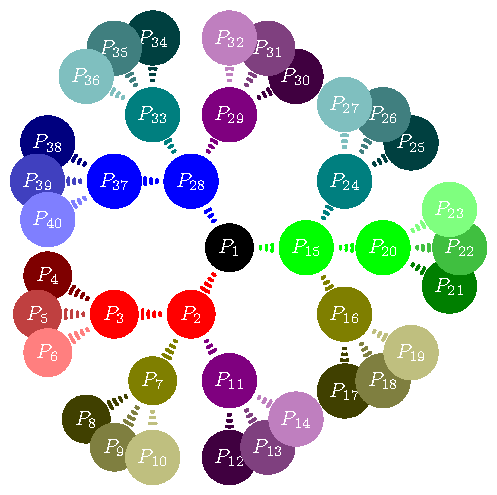
\includegraphics[width=.35\textwidth]{grafoMEW.pdf}
	\caption[Estructura del sitio web]{\small Estructura del sitio web}
	\label{fig:grafoMEW}
\end{wrapfigure}
En muchos sitios web existe una página denominada "`mapa del sitio"'. Se trata generalmente de un listado de las páginas de $P$ organizado según los criterios del diseñador del mapa y que no considera los enlaces de $E$ creados dinámicamente. Puede reorganizarse dinámicamente si cada página contiene metadatos con palabras clave asociadas a su contenido, pero conforme aumenta el número de páginas de $P$ se va haciendo más difícil su correcta gestión y acaba por ser un mapa pobremente actualizado.

Si el sitio web es de pequeñas dimensiones es muy fácil representar su estructura mediante un \grafo, sin embargo si es un sitio web con muchas páginas visitables y muy dinámico en su contenido acaban siendo tan grandes los \grafos que dejan de aportar información. La \wsm puede ayudar mucho en este aspecto al desarrollador del sitio web, mostrándole \grafos similares al de la figura~\ref{fig:grafoMEW} simplemente leyendo una página del sitio web y recorriendo todos sus enlaces internos, permitiéndole centrarse en \grafos más pequeños generados de forma dinámica.





En la fase de preproceso hemos obtenido un \flog reducido en que sólo aparecen las solicitudes de páginas realizadas por los usuarios del sitio web, lo que en la literatura se conoce como \emph{clickstream}~\citep{BucklinSismeiro-AModelOfWebSiteBrowsing-2001}, junto con el resto de variables seleccionadas para el análisis (IP del solicitante, fecha, hora, estado\ldots). Con los \emph{clickstreams} sólo sabemos \emph{qué} visitan los usuarios en nuestro sitio web pero no \emph{cómo} lo hacen. Hemos de utilizar un modelo de datos que represente el comportamiento de un usuario de un sitio web, siendo la \sn un buen punto de partida. Una \sn es una \secuencia de interacciones entre el usuario y un sitio web que podría ser generalizada del siguiente modo:
\begin{enumerate}
	\item El usuario tiene un objetivo (o varios) que le llevan a entrar en nuestro sitio web.
	\item Si no encuentra directamente lo que busca se fija en los enlaces existentes en la página en que está, siempre que su diseño doten de usabilidad a dichos enlaces, o incluso utiliza \texttt{Ctrl+F} para buscar en la página pistas sobre su objetivo.\label{item:2-definicion-sesion}
   \item Si no encuentra nada puede volver a la página anterior (con \texttt{Alt+$\leftarrow$ o \texttt{Retroceso}}, con lo que no solicita nada al servidor pues suele estar guardada en la caché de cliente) o bien puede dar por terminada su \sn.
	\item Si encuentra un enlace a otra página de nuestro sitio web que le parece el camino más apropiado para cumplir con su objetivo lo utilizará, solicitando una nueva página en su sesión. Vuelve a encontrarse en la situación planteada en el punto~\ref{item:2-definicion-sesion}.
   \item Si no encuentra nada su \sn ha terminado.
\end{enumerate}

En el \flog reducido no se refleja por qué ha abandonado la sesión el usuario, y si se ha usado la caché del cliente es posible que se encuentren situaciones no previstas en el sitio web si la siguiente página registrada por el usuario en el \flog no puede provenir de la página actual por no existir el enlace. Sólo si está registrado y ha iniciado sesión identificada en el sitio web podemos recabar información sobre su navegación real, concretamente sobre la finalización de la sesión. Puede abandonar nuestro sitio web satisfecho por haber encontrado fácilmente su objetivo o bien incómodo por haber perdido el tiempo buscándolo en nuestro sitio web. Como lo que queremos es descubrir cómo usan nuestro sitio web vamos a plantear como primera hipótesis que los usuarios abandonan el sitio web satisfechos por haber encontrado en la última página de su \sn el objetivo que tenía desde el principio. Se supone que los usuarios que vuelven a nuestro sitio web es porque les ha resultado útil y es su comportamiento el que estamos analizando, cada vez con más datos. Los usuarios que no vuelven acaban por dejar de encajar en los \patrones de navegación que hayamos descubierto y sus datos acabarán por ser ignorados por los algoritmos de \DM.

% Este proceso puede ser cíclico hasta que el usuario encuentra su objetivo y abandona satisfecho nuestro sitio web o bien decide que será mejor buscarlo en otro sitio web. Sólo en sitios webs específicos sabremos que el usuario ha encontrado realmente su objetivo (en una tienda electrónica tras hacer efectiva una compra, por ejemplo), esa información no la encontraremos en casi ningún \flog. A pesar de ello lo que ahora realmente nos interesa es buscar \patrones de comportamiento entre los usuarios de nuestro sitio web por lo que no tendremos en cuenta si el usuario ha logrado finalmente su objetivo, sólo tendremos en cuenta de qué modo "`navega"' a través de nuestro sitio web. Lo que podemos observar del usuario es una \secuencia de clickstreams, conocido también como \sn.

Para estudiar el comportamiento de nuestros usuarios hay que construir las \sns de cada uno de ellos, agrupando adecuadamente todos los clickstreams que haya producido, considerando que cada usuario está identificado por la IP utilizada. La asociación usuario-IP no es totalmente correcta pues debido a las características de las redes internas de comunicación es posible que diferentes usuarios utilicen la misma IP, además de existir las IPs dinámicas, un mismo usuario podría usar diferentes IPs en sus visitas al sitio web, más hoy en día que puede acceder a la \WWW desde múltiples lugares y dispositivos. Si no hay un registro efectivo del usuario no podemos identificarlo unívocamente, sin embargo la solución tomada es la máxima información que podremos extraer de \flogs anónimos.

Un problema que presenta la obtención de \sns es que no suele haber información precisa sobre las mismas en el \flog ya que el protocolo \texttt{html} carece de estado. Los usuarios de un sitio web son en su mayoría anónimos por lo que la finalización de una \sn se determina de forma heurística. Se han propuesto diversas alternativas: fijando un umbral a la duración máxima de una sesión (2, 4 u 8 horas, p.ej.), o al intervalo de tiempo máximo entre dos clickstream consecutivos (10 o 30 minutos, p.ej.), o una combinación de ambas, o incluso si ya se tienen clasificadas las páginas del sitio web en diferentes temáticas un cambio de temática podría interpretarse como un final de sesión. Existen muchos trabajos que abordan este tema (\cite{HeGoker-DetectingSessionBoundaries-2000,HuangPengAnSchuurmansCercone-SessionBoundaryDetection-2003}; Huang, Peng, An y Schuurmans, \cite*{HuangPengAnSchuurmans-DynamicWebLogSessionBoundaryDetection-2004}, \cite*{HuangPengAnSchuurmans-DynamicWebLogSessionIdentification-2004}).

\begin{Definition}[\Sn]\label{def:1-2-4-sesion}
  Una \sn es un vector ordenado de las páginas visitadas por un usuario en un intervalo de tiempo determinado por $maxClick$ y $maxSession$ con información sobre el tiempo transcurrido entre la visita de cada par de páginas del vector
  \begin{equation}\label{eq:1-2-4-primerasSesiones}
    s_i = \left({userID}, p_1, u_1, p_2, u_2\ldots p_{n_i-1}, u_{n_i-1}, p_{n_i}\right)
  \end{equation}
\end{Definition}

Con este procedimiento obtendremos $N$ vectores como el expuesto en la ecuación~\ref{eq:1-2-4-primerasSesiones}, donde $i$ enumera las diferentes sesiones, $userID$ identifica al usuario que ha hecho la solicitud, $p_j$ representa la página solicitada y $u_j$ el tiempo que permanece en ella o, mejor dicho, el tiempo transcurrido entre la solicitud de la página $p_j$ y la de $p_{j+1}$ (realmente no sabemos qué hizo el usuario durante ese tiempo). $n_i$ es el número de páginas visitadas en la sesión $i$-ésima, con lo que el número de registros del \flog reducido coincide con $\sum_{i=1}^N{n_i}$. Nótese que desconocemos $u_{n_i}$ pues tras la visita de la página $p_{n_i}$ finaliza la sesión, si quisiéramos usar el tiempo de permanencia en todas las páginas de una sesión deberíamos estimar $u_{n_i}$.

\begin{Definition}[Conjunto de \sns]\label{def:1-2-4-cjto-sesion}
  Sea $S$ el conjunto de todas las \sns obtenidas tras la fase de transformación
  \begin{equation}\label{eq:1-2-4-cjto-sesiones}
    S = \left\{s_i, i = 1\ldots N\right\}
  \end{equation}
\end{Definition}

% \afterpage{\clearpage}
\lstinputlisting[style=miSQL,
                       label=listado:crearSesiones,
                       caption={Algoritmo de obtención de \sns}]
                       {./contenido/srw/codigo/algCrearSesiones}

El algoritmo para obtener las \sns a partir del \flog reducido (véase el listado~\ref{listado:crearSesiones}) no es costoso computacionalmente hablando. En nuestros primeros experimentos utilizamos una duración máxima de sesión de 4 horas y un intervalo máximo de 30 minutos entre dos clickstreams para considerar que una sesión ha finalizado. En el pseudocódigo del algoritmo se utilizan los valores $maxSession$ y $maxClick$ para referirnos a estos umbrales respectivamente.

La función $CreaSesion()$ recibe como parámetro los tres valores recogidos en el $registro$ en que nos encontramos, crea la nueva sesión y la incorpora al conjunto de sesiones abiertas. Como aún no sabemos cuánto tiempo permanece en la página $p_i$ usaremos dos variables auxiliares que marcarán el inicio y fin de la sesión mientras la estamos construyendo, en este caso $t_i$.

\lstinputlisting[style=miSQL,
                       label=listado:funcion-CreaSesion,
                       caption={Función $CreaSesion()$}]
                       {./contenido/srw/codigo/funCreaSesion}

La función $CierraSesion()$ recibe como parámetro la sesión que ha de cerrarse, a la que se eliminan los datos auxiliares $t_0$ (inicio de sesión) y $t_{fin}$ (fin de sesión). Estos datos podrían guardarse si van a ser utilizados en las siguientes fases del proceso de \WUM, para seleccionar sesiones en función de su horario, día de la semana, temporada\ldots En nuestro caso no los utilizamos por lo que podemos prescindir de ellos. Finalmente, la función mueve la sesión del conjunto de sesiones abiertas al conjunto de sesiones, resultado final del algoritmo.

\lstinputlisting[style=miSQL,
                       label=listado:funcion-CierraSesion,
                       caption={Función $CierraSesion()$}]
                       {./contenido/srw/codigo/funCierraSesion}

Mediante esta transformación ya tenemos los datos modelados en función de lo que estamos buscando: conocer el comportamiento de los usuarios de nuestro sitio web para aprender a sugerir a un usuario las páginas que podría estar buscando en función de las páginas que está visitando en tiempo real. Esta fase consiste, pues, en transformar datos crudos en estructuras que modelen mejor a los individuos que queremos estudiar, en este caso las \sns de los usuarios de un sitio web.

\begin{wrapfigure}{o}{0.45\textwidth}
  \centering
  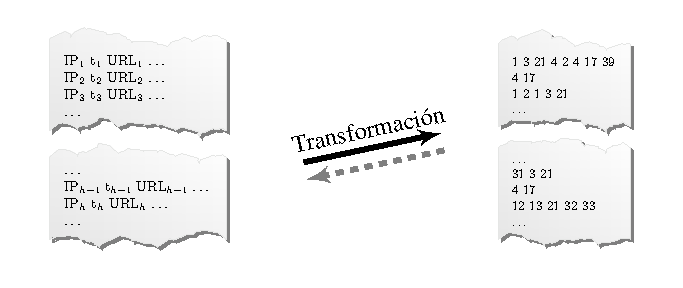
\includegraphics[width=.45\textwidth]{Transformacion.pdf}
	\caption{Transformación}
	\label{fig:Transformacion}
\end{wrapfigure}
En la siguiente fase se transformarán de nuevo de los datos, esta vez para adaptarlos a los algoritmos de \dm a los que serán sometidos. Ya tenemos los datos transformados y guardados mediante una estructura que es fácil de describir usando gran variedad de métodos estadísticos de análisis de datos en casi cualquier dispositivo informático.

La Estadística y la Informática llevan muchos años trabajando conjuntamente, con las aportaciones de otras ciencias, en extraer información más o menos compleja de cualquier colección de datos estructurada. Podríamos realizar complejos análisis estadísticos a las \sns que tenemos pero estamos en un proceso de \wum y usaremos estos datos con técnicas de \dm. Podemos realizar sencillos análisis estadísticos descriptivos sobre los datos que tenemos. Sencillos porque a pesar de haber seleccionado, preprocesado y transformado los datos consiguiendo una enorme reducción respecto a la cantidad de datos iniciales aún tenemos muchos datos. Si observamos qué datos tenemos almacenados en las \sns es fácil obtener conocimiento básico sobre las páginas visitadas por los usuarios del sitio web.






Nosotros estamos trabajando desde la perspectiva de la \WUM por lo que nos centraremos en la información que tenemos sobre el uso del sitio web, las \sns. Es inmediato deducir que podemos extraer dos nuevos conjuntos de datos, para conocer qué páginas de $P$ y qué enlaces de $E$ se utilizan en realidad en nuestro sitio web. De hecho el conjunto de páginas visitadas lo podríamos obtener antes de haber creado las \sns.

\begin{Definition}[\emph{Páginas visitadas} del sitio web]\label{def:1-2-4-cjto-paginasVisitadasSW}
   Sea $P' \subseteq P$ el conjunto de todas las páginas visitadas en el sitio web y $flog_{red}$ el \flog reducido.
  \begin{equation}\label{eq:1-2-4-cjto-paginasVisitadasSW}
     P' = \left\{P_i \in P \ | \ P_i \in flog_{red}\right\} = \left\{P_i \in P \ | \ P_i \in S\right\}
  \end{equation}
\end{Definition}

El primer análisis que se puede llevar a cabo es el estudio de $\neg P'$, las páginas de $P$ que nunca visitan nuestros usuarios. Si son irrelevantes o su contenido ya está en otra página de $P'$ sería bueno eliminarlas, junto a los enlaces que apuntan a ellas, para reducir las dimensiones del sitio web sin perder su verdadera utilidad, ganando en usabilidad. Si son importantes habrá que plantear si debe mejorarse $E$ o simplemente mejorar el texto de los mensajes de los enlaces que apuntan a estas páginas para que sean comprendidos por los usuarios del sitio web. Deben anotarse para poder comprobar en futuros análisis del sitio web si ha tenido efecto el cambio realizado.

La frecuencia de uso de cada página, $N_i$, es un indicador de su popularidad, pero aún no sabemos si una página es popular por ser el \emph{objetivo} de muchos de nuestros usuarios o simplemente lo es como página de \emph{transición} entre otras páginas. Si el conocimiento adquirido al final del proceso de \WUM se integra adecuadamente se podrá observar un cambio en estas frecuencias, en tal caso es posible que páginas que sólo se usan como \emph{transición} desaparecen de muchas las nuevas \sns.

\begin{Definition}[Tiempo de permanencia en las \emph{páginas visitadas}]\label{def:1-2-4-tiempoPermanencia:paginasVisitadasSW}
   Sea $\overrightarrow{u}_i$ el conjunto de tiempos de permanencia en la página $P_i$.
  \begin{equation}\label{eq:1-2-4-tiempoPermanencia}
    \overrightarrow{u}_i = \left(u_{1}, \ldots u_{N_i}\right)
  \end{equation}
\end{Definition}

En $\overrightarrow{u}_i$ guardamos el tiempo de permanencia de algunas de las $N_i$ visitas que ha recibido la pagina $P_i$. Si $P_i$ es la última página de una \sn no sabemos cuánto tiempo ha permanecido el usuario en esa página durante esa sesión por lo que no es un dato que conozcamos. Se pueden hacer rápidas estimaciones a partir de \overrightarrow{u_i}. Su media, moda o intervalos de confianza podrían darnos información sobre el uso de las páginas del sitio web y orientarnos hacia la siguiente fase, la aplicación de una técnica de \DM para extraer conocimientos más profundos sobre los datos en estudio.

El conjunto de enlaces de $E$ realmente utilizados por nuestros usuarios forma parte de la información que contienen las \sns.

\begin{Definition}[\emph{Enlaces internos utilizados} en el sitio web]\label{def:1-2-4-cjto-enlacesInternosUsados}
   Sea $E' \subset E$ el conjunto de todos los enlaces internos \emph{utilizados} por los usuarios del sitio web. Se define $E'_{jk}$ cuando existe alguna sesión que contiene la secuencia $P_j, n_j, P_k$.
  \begin{equation}\label{eq:1-2-4-cjto-enlacesUsados}
    E' = \left\{E_{jk} \in E,\ | \ \exists s_i \in S \ | \ (P_j, n_j, P_k) \in s_i,\ j\neq k,\ j,k\in\{1\ldots M\}\right\}
  \end{equation}
\end{Definition}

La comparación entre $E$ y $E'$ nos permitirá preguntarnos por qué no se usan los enlaces de $\neg E'$. Para reducir las dimensiones de $\neg E'$ basta con aplicar lo que ya podemos inferir de $P'$, que si $P_i \notin P' \Leftarrow E_{ij} \wedge E_{ji} \notin E'$. El uso de enlaces está estrechamente relacionado con el uso de las páginas del sitio web, la mayoría de información obtenida al analizar $P'$ coincidirá con la obtenida al analizar $E'$, sin embargo en $E'$ podemos observar la relación encontrada por los usuarios entre las páginas de nuestro sitio web sin recurrir a técnicas de \DM.

El número de visitas recibidas por la página $P_k$, $N_k$, será mayor o igual al número de enlaces de $E'$ que conduzcan a la página $P_k$. Sólo coincidirán cuando la página $P_k$ no sea nunca la primera página visitada en una sesión.

La transformación hecha a los datos nos hace comprender mejor lo que estamos estudiando pero aún son muchos datos y no basta con análisis descriptivos para extraer el conocimiento que contienen. En la siguiente fase se abre un gran abanico de posibilidades, ya sabemos qué datos tenemos, cuántos son, podemos preguntarnos qué conocimiento contienen desde diferentes perspectivas y aplicando nuevas transformaciones a nuestro modelo para conseguir datos más adaptados a las herramientas que usaremos para su análisis.
